\documentclass{beamer}
\usepackage{fontspec}
\usepackage{beamerthemeshadow}
\usepackage{mathtools}
\begin{document}
\newcommand{\fastq}{\textit{fastq}}
\begin{frame}{\textit{Fastq} file format}
	$\underbrace{@SFHMR:01926:02303}_\text{Read ID}$
	\pause 
	$\underbrace{GAGACCCGCATCGCCATCTTGCGCAAGAAAGCACAGATG}_\text{DNA sequence}$
	\pause
	$\underbrace{+}_\text{A plus}$
	\pause
	$\underbrace{??>>3D<;<@@BB9??@;6>999?9CC:DCB>>?BBBB<}_\text{Nucleotide qualities}$
\end{frame}
\begin{frame}{\textit{Fastq} file format}
\framesubtitle{Quality}

\includegraphics[width=8cm, keepaspectratio]{pic/fq_qual.png} \\
Nucleotide G has a quality of ?
%paturpināt 
\end{frame}

\begin{frame}{Deciphering of quality "?"}
%\framesubtitle{}
Symbol $\rightarrow$ Encoded value $\rightarrow$ Quality score $\rightarrow$ Probability of error
\end{frame}

\begin{frame}{Deciphering of quality "?"}
\framesubtitle{Symbol $\rightarrow$ Encoded value}
\end{frame}

\begin{frame}{Deciphering of quality "?"}
\framesubtitle{Symbol $\rightarrow$ Encoded value}
http://www.ascii-code.com/ \\
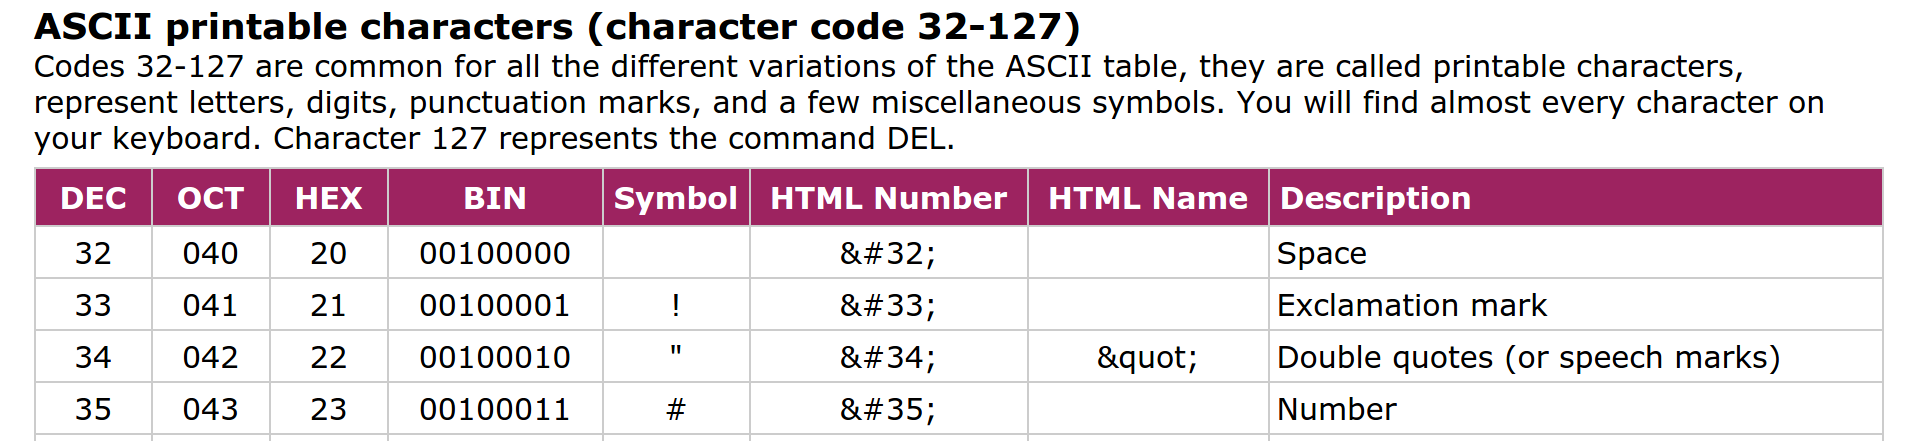
\includegraphics[width=\linewidth, keepaspectratio]{pic/ascii_head3.png} \\
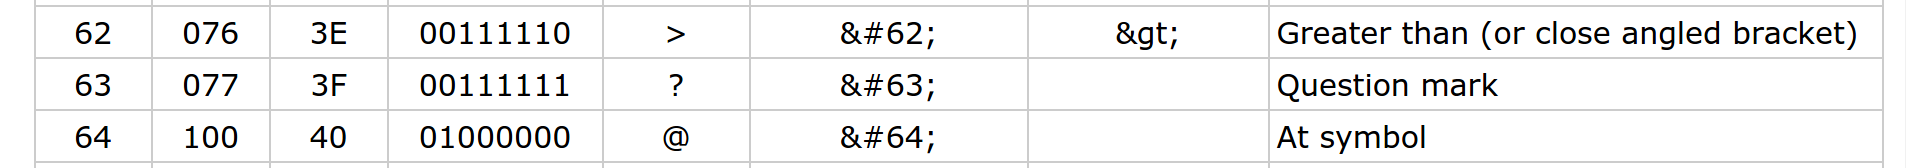
\includegraphics[width=\linewidth, keepaspectratio]{pic/ascii_tail3.png} \\
\end{frame}

\begin{frame}{Deciphering of quality "?"}
\framesubtitle{Encoded value $\rightarrow$ Quality score}
By looking at ascii table we found out that symbol ? is encoded as a decimal value 63
Symbols used for quality score encoding (Sanger) start with symbol ! (encoded as decimal value 33)
To obtain the quality score (also known as Phred quality score) we need to substract smallest possible value (33) from the obtained value 63.
63 - 33 = 30
\end{frame}

\begin{frame}{Deciphering of quality "?"}
\framesubtitle{Quality score $\rightarrow$ Probability of error}
$p = 10^{-\frac{Q}{10}}$ \\
Our Q = 30, therefore\\
$p = 10^{-\frac{30}{10}} = 10^{-3} = 0.001$ \\
Probability that nucleotide G is an error = 0.001
\end{frame}
\begin{frame}{\textit{Fastq} quality control}
\framesubtitle{Assessment of quality}
http://www.bioinformatics.babraham.ac.uk/projects/fastqc/
\end{frame}

\begin{frame}{\textit{Fastq} quality control}
\framesubtitle{Trimming and filtering of reads}
http://www.bioinformatics.babraham.ac.uk/projects/fastqc/
\end{frame}

\begin{frame}{\textit{Fastq} quality control}
\framesubtitle{Repeated assessment of quality}
http://www.bioinformatics.babraham.ac.uk/projects/fastqc/
\end{frame}

{
\usebackgroundtemplate{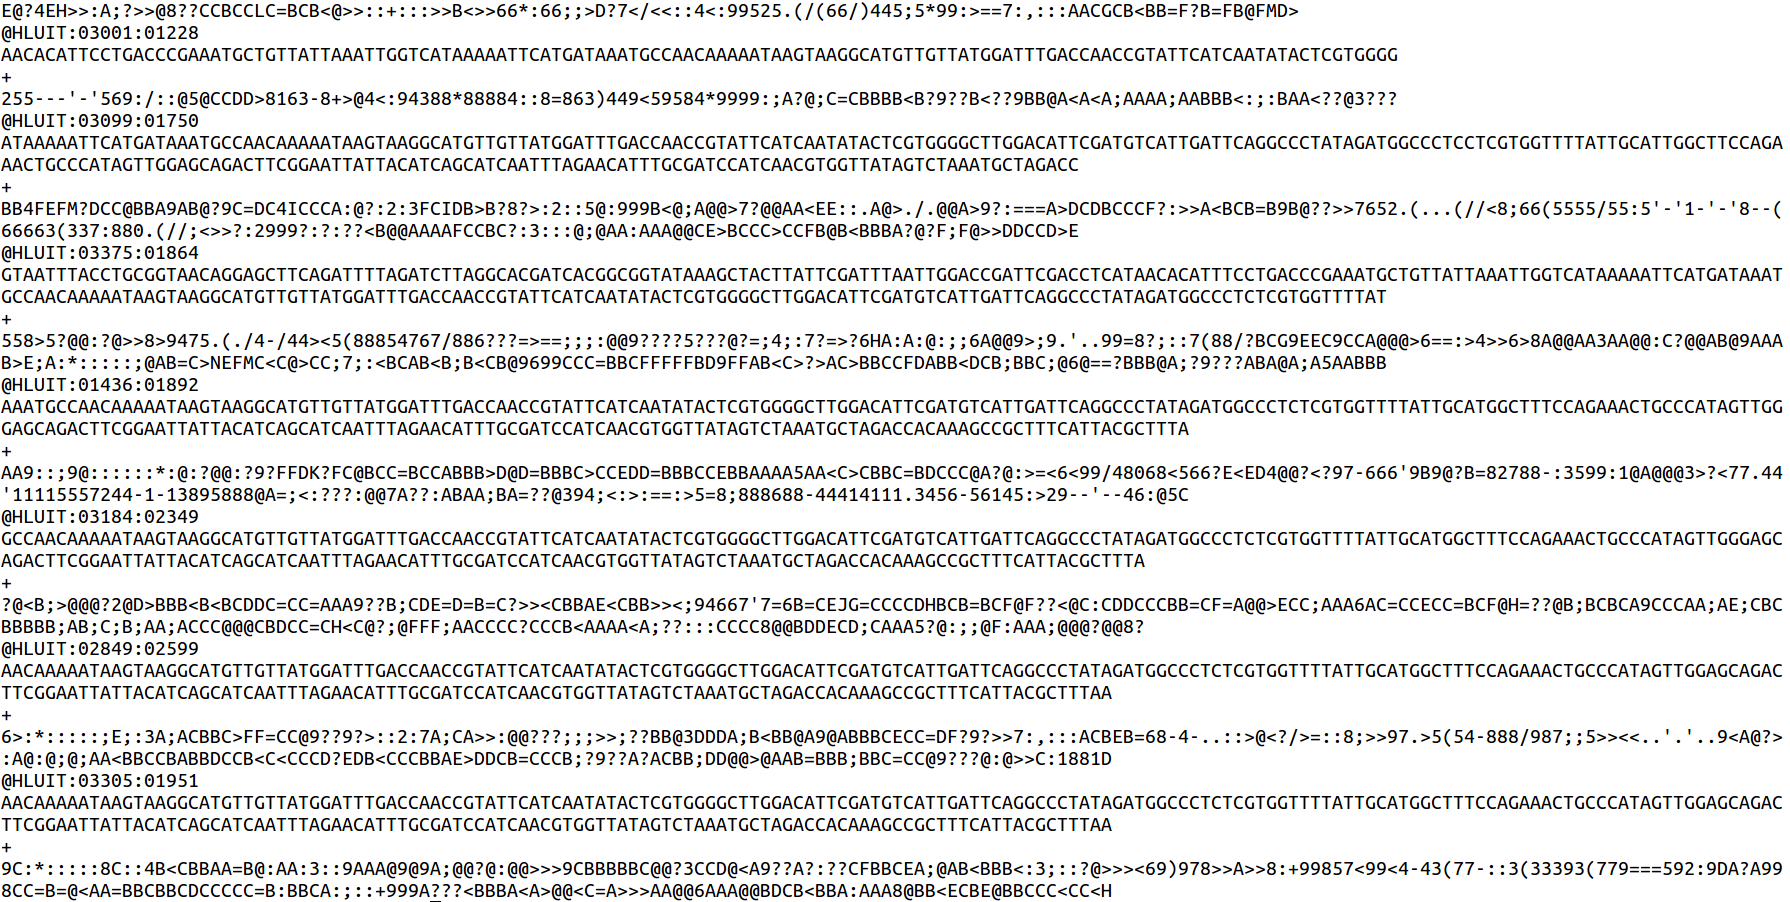
\includegraphics[width=\paperwidth, height=\paperheight]{pic/readi.png}}
\begin{frame}[plain]
\end{frame}
}
\end{document}
